\title{\textbf{CSCI 203 Place-out Project} \\
\texttt{final.pdf}
    \vspace{-6mm}}
\documentclass[12pt,letterpaper]{article}

\usepackage[utf8]{inputenc}
\usepackage [english]{babel}
\usepackage [autostyle, english = american]{csquotes}
\MakeOuterQuote{"}

\usepackage[margin=1in]{geometry}
\usepackage{setspace}
\setlength{\parindent}{0.2in}
\setlength{\parskip}{6pt}

%% To insert images and URLs (for Bibliography) %%
\usepackage{graphicx}
\usepackage[hyphens]{url}

%% To edit header %%
\usepackage{fancyhdr}
\pagestyle{fancy}
\fancyhead{}
\lhead{Yash Mittal}

%% To insert code (set format) %%
\usepackage{listings}
\lstset{
  aboveskip=2mm,
  belowskip=2mm,
  showstringspaces=false,
  columns=flexible,
  basicstyle={\small\ttfamily},
  numbers=none,
  breaklines=true,
  breakatwhitespace=true,
  tabsize=4
}

%% To reduce Top Margin to 1 inch only %%
\usepackage{etoolbox}
\makeatletter
\patchcmd{\@maketitle}
  {\null\vskip 2em\begin{center}}
  {\centering}
  {}
  {}
\patchcmd{\@maketitle}
  {\end{center}}
  {}
  {}
  {}
\makeatother

\begin{document}

\date{}
\maketitle
\vspace{-12mm}

\setstretch{1.0}
\thispagestyle{fancy}

For the final part of \texttt{CSCI 203} final project, I implemented a web crawler, drawing inspiration from what I learned during an online course \texttt{CS101}: Building a Search Engine. The web crawler collects the text from all web pages with links present on the user-entered \texttt{URL}. The process continues until \texttt{DEPTH} number of "hops" from the original page are made. For example, only the first web page is crawled if \texttt{DEPTH} is set to \texttt{0}. However, even the pages linked from that page are searched if \texttt{DEPTH} is increased to \texttt{1}. A simple \texttt{if} statement is used to ensure that all pages are visited exactly once.

I revamped the program \texttt{simpleTextCloudDisplay.py} to create a more organized text cloud. The modified program named as \texttt{complexTextCloudDisplay.py} has the following functions:

\vspace{-4mm}
\begin{itemize}
    \item \texttt{windowSetup()} \\
        Sets up the \texttt{VPython} window "scene"
    \item \texttt{extreme(freqList, max\textunderscore min)} \\
        Returns position of maximum frequency if \texttt{max\textunderscore min} is \texttt{True}, position of minimum frequency otherwise
    \item \texttt{findHeight(freqList, pos)} \\
        Returns height (font size) of a word on position \texttt{pos}
    \item \texttt{findWidth(freqList, pos)} \\
        Returns approximate "screen width of word" on position \texttt{pos}
    \item \texttt{displayCloud(freqList)} \\
       Invokes \texttt{windowSetup()} and displays a Text Cloud 
\end{itemize}

Furthermore, I polished the \texttt{stemContent()} by including a \texttt{Dict} named as \texttt{exceptions}. The stemming process is bypassed for any word which is one of the keys in \texttt{exceptions}, and its corresponding value is then treated as the stemmed word. Following is a sample program output with \texttt{MAX\textunderscore WORDS} and \texttt{DEPTH} set to \texttt{50} and \texttt{2} respectively:

{\centering
    \fbox{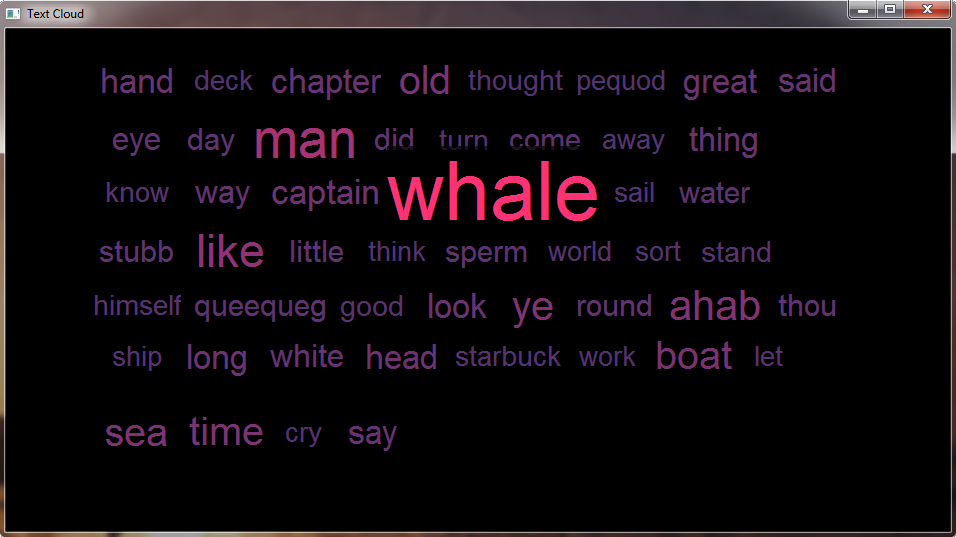
\includegraphics[scale=0.35]{output}} 
\par}

\begin{lstlisting}
    Please enter a URL http://www.eg.bucknell.edu/~csci203/common-files/sampleText/moby-dick.html
    [(`whale', 1392), (`man', 762), (`like', 588), (`ahab', 498), (`ye', 486), (`sea', 466), (`old', 446), (`time', 436), (`boat', 426), (`captain', 337), (`head', 333), (`hand', 329), (`look', 326), (`long', 324), (`great', 324), (`chapter', 315), (`thing', 312), (`say', 311), (`said', 293), (`way', 278), (`white', 276), (`eye', 268), (`thou', 264), (`stubb', 257), (`round', 256), (`did', 251), (`little', 249), (`day', 248), (`sperm', 241), (`queequeg', 239), (`water', 231), (`come', 226), (`turn', 213), (`stand', 203), (`good', 203), (`himself', 200), (`know', 194), (`starbuck', 189), (`sail', 186), (`thought', 183), (`let', 183), (`deck', 181), (`world', 177), (`away', 176), (`pequod', 175), (`work', 172), (`ship', 172), (`sort', 171), (`think', 169), (`cry', 166)]
\end{lstlisting}

\vspace{4mm}
\hrule

\renewcommand{\labelenumii}{\roman{enumii}.}
\begin{enumerate}
    \item Following are three functions which can be reused in similar programs:
        \begin{itemize}
            \item \texttt{ModifiedStemmer.stem()} \\
                Most search engine crawl web pages for specific information. This function could be used in a web search engine algorithm to remove suffixes from query words. Such a function would even list the otherwise neglected results.
            \item \texttt{complexTextCloudDisplay.displayCloud()} \\
               This function could be put to use whenever a visual display is needed. Facebook and Twitter could implement such a method to display a text cloud of all trending topics wherein each topic link to a corresponding news feed.
            \item \texttt{project\textunderscore part1.getContent()} \\
                If a website does not provide an Application Program Interface (API), this function could be used for basic web scraping, which means to extract useful information from web pages.
        \end{itemize}
        
        I enjoyed implementing a couple of program features. First of all, the \texttt{ModifiedStemmer Class} definition uses slick logic to minimize the lines of code while accounting for most major suffixes. Even though \texttt{stemMajor()} function is a bit hard to read, the overall efficiency of my stemmer is on a higher side.
        
        Throughout the program, I try to optimize space complexity. In \texttt{cleanContent()}, \texttt{stopwordsIndices} maintains the indices of stopwords in \texttt{wordList}. Instead of appending to \texttt{stopwordsIndices} though, a stopword index is inserted at its beginning. This avoids \texttt{IndexError} as the program deletes stopwords from right to left. Additionally, I make local copies of \texttt{MAX\textunderscore WORDS} and \texttt{DEPTH} so that the program does not encounter errors due to \texttt{global} variables.
        
    \item After testing my program files multiple times, I feel that a considerable portion of this project should be working fine. Though there could be several "doom scenarios" that could result in anomalous behavior. If the web crawler encounters \texttt{www.bucknell.edu} or any similar generic \texttt{URL} with massive number of links, the program can take a lot of time to gather content and may even cause the program to crash due to excessive memory use.
    
    Also, randomization of \texttt{freqList} in \texttt{displayCloud()} could result in undesirable spacing in the following case. If a word is among the more frequent words in \texttt{freqList} and is to be put at the beginning of a line, the resulting window scene would have unwanted space before that particular line.
    
    \item Given more time, following features could be incorporated to my project:
        \begin{itemize}
            \item Improve display by using a \texttt{Tkinter Canvas} instead of \texttt{Labels}. While searching for documentation on \texttt{scene} and \texttt{Label}, I discovered that \texttt{Canvas} would be simpler to display a Text Cloud and would subsequently reduce hard-coding coordinate values.
            \item Account for more suffixes in \texttt{ModifiedStemmer Class}. In the original paper by Martin Porter, there are five levels of stemming, last two of which cover less prominent suffixes. Efficiency of my stemmer could be further increased if these suffixes are considered too.
            \item Make the program more user-friendly. This can be done by outputting helpful messages throughout program run. For instance, if a user enters an invalid \texttt{URL} at first, a message asking if (s)he would like to continue with the program and enter another \texttt{URL} could go a long way.
        \end{itemize}
\end{enumerate}

%% Bibliography %%

\renewcommand\refname{References \textit{\&} Useful Links}
\bibliographystyle{unsrt}
\bibliography{references.bib}
\nocite{*}

\end{document}